\section{Simulation of Summarization Score}

\begin{figure}
    \caption{Simulation of Summarization Score\label{fig:simulation_of_score}}
    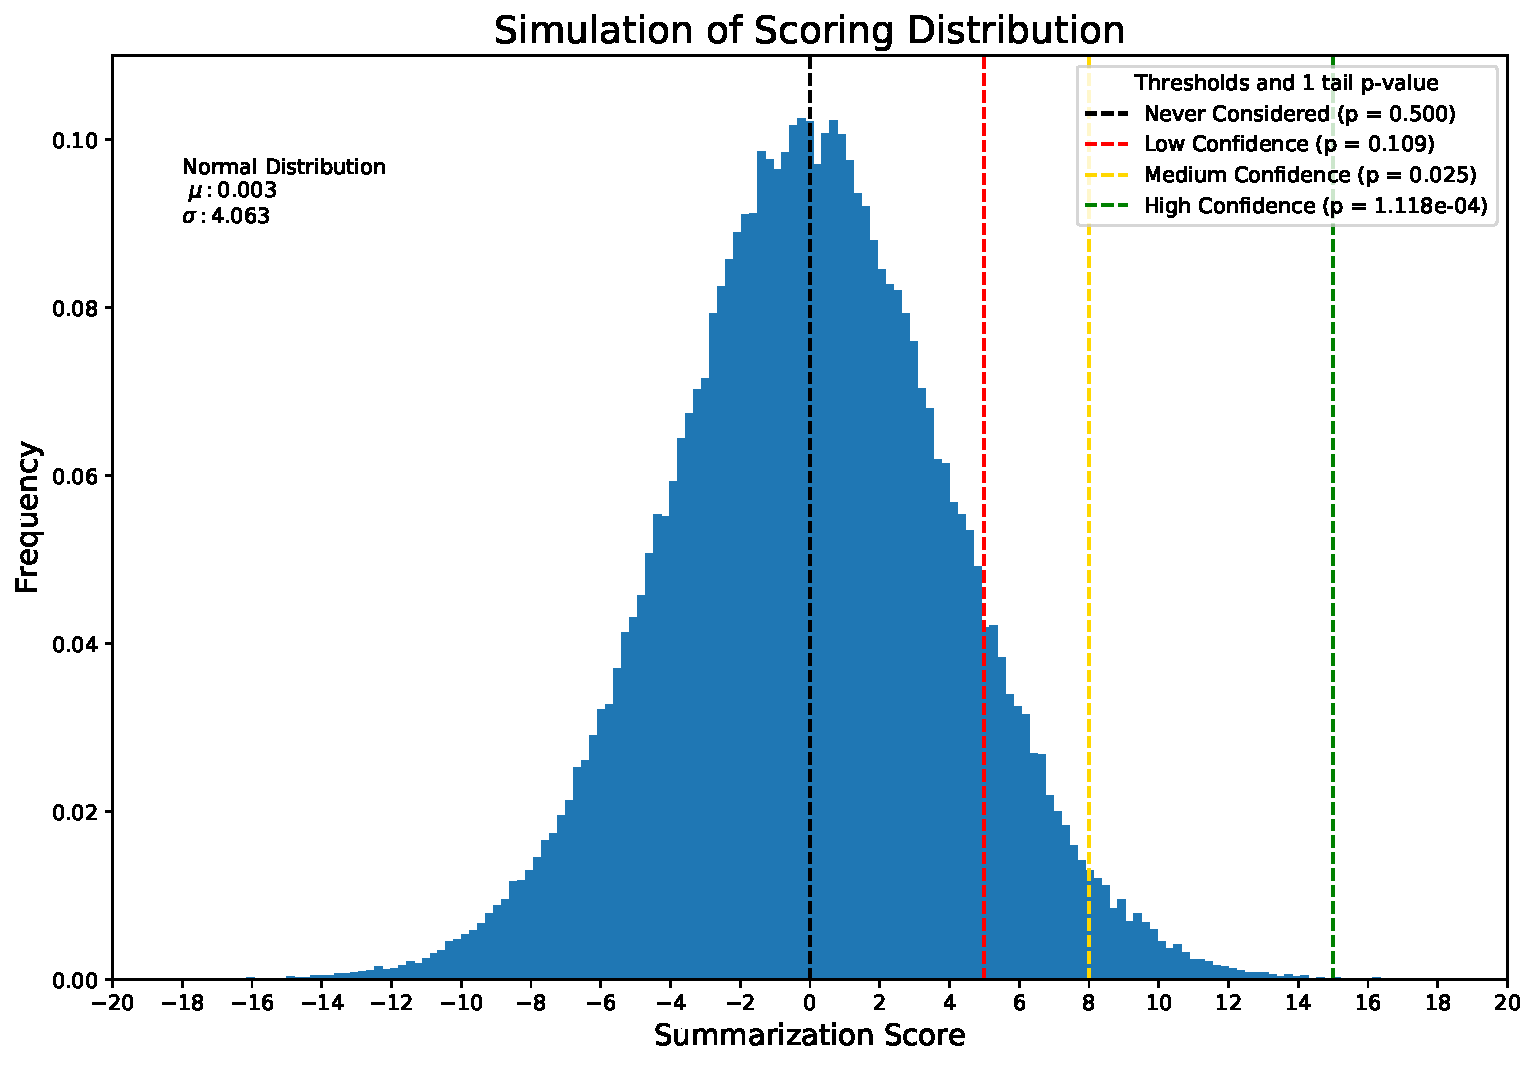
\includegraphics[width=.95\linewidth]{figure/simulation_of_scoring_distribution.pdf}
\end{figure}

To simulate the summarization score, we assume that each component scoring feature is
drawn from an independent uniform distribution. We sample these five distributions
100,000 times, and for each set of five feature scores compute $\sum_j\text{logit}(f_{i, j})$.
According to the central limit theorem, the distribution of the summarization score should be
normal, with a mean at approximately 0. We noted two score thresholds, 8 and 15 for lower
confidence and high confidence matches. We connect these score thresholds to p values from
one-sided tests for significance from thes simulated distribution. The threshold of $8$ has
a p value of $\sim0.025$, while $15$ has a p value of $\sim1.1\times10^{-4}$.